% Options for packages loaded elsewhere
\PassOptionsToPackage{unicode}{hyperref}
\PassOptionsToPackage{hyphens}{url}
%
\documentclass[
  english,
  man]{apa6}
\usepackage{lmodern}
\usepackage{amssymb,amsmath}
\usepackage{ifxetex,ifluatex}
\ifnum 0\ifxetex 1\fi\ifluatex 1\fi=0 % if pdftex
  \usepackage[T1]{fontenc}
  \usepackage[utf8]{inputenc}
  \usepackage{textcomp} % provide euro and other symbols
\else % if luatex or xetex
  \usepackage{unicode-math}
  \defaultfontfeatures{Scale=MatchLowercase}
  \defaultfontfeatures[\rmfamily]{Ligatures=TeX,Scale=1}
\fi
% Use upquote if available, for straight quotes in verbatim environments
\IfFileExists{upquote.sty}{\usepackage{upquote}}{}
\IfFileExists{microtype.sty}{% use microtype if available
  \usepackage[]{microtype}
  \UseMicrotypeSet[protrusion]{basicmath} % disable protrusion for tt fonts
}{}
\makeatletter
\@ifundefined{KOMAClassName}{% if non-KOMA class
  \IfFileExists{parskip.sty}{%
    \usepackage{parskip}
  }{% else
    \setlength{\parindent}{0pt}
    \setlength{\parskip}{6pt plus 2pt minus 1pt}}
}{% if KOMA class
  \KOMAoptions{parskip=half}}
\makeatother
\usepackage{xcolor}
\IfFileExists{xurl.sty}{\usepackage{xurl}}{} % add URL line breaks if available
\IfFileExists{bookmark.sty}{\usepackage{bookmark}}{\usepackage{hyperref}}
\hypersetup{
  pdftitle={An institutional approach to attention allocation and venture resource mobilization and acquisition},
  pdfauthor={Ouafaa Hmaddi1},
  pdfkeywords={attention, resources, institutional capital, accelerators},
  hidelinks,
  pdfcreator={LaTeX via pandoc}}
\urlstyle{same} % disable monospaced font for URLs
\usepackage{graphicx,grffile}
\makeatletter
\def\maxwidth{\ifdim\Gin@nat@width>\linewidth\linewidth\else\Gin@nat@width\fi}
\def\maxheight{\ifdim\Gin@nat@height>\textheight\textheight\else\Gin@nat@height\fi}
\makeatother
% Scale images if necessary, so that they will not overflow the page
% margins by default, and it is still possible to overwrite the defaults
% using explicit options in \includegraphics[width, height, ...]{}
\setkeys{Gin}{width=\maxwidth,height=\maxheight,keepaspectratio}
% Set default figure placement to htbp
\makeatletter
\def\fps@figure{htbp}
\makeatother
\setlength{\emergencystretch}{3em} % prevent overfull lines
\providecommand{\tightlist}{%
  \setlength{\itemsep}{0pt}\setlength{\parskip}{0pt}}
\setcounter{secnumdepth}{-\maxdimen} % remove section numbering
% Make \paragraph and \subparagraph free-standing
\ifx\paragraph\undefined\else
  \let\oldparagraph\paragraph
  \renewcommand{\paragraph}[1]{\oldparagraph{#1}\mbox{}}
\fi
\ifx\subparagraph\undefined\else
  \let\oldsubparagraph\subparagraph
  \renewcommand{\subparagraph}[1]{\oldsubparagraph{#1}\mbox{}}
\fi
% Manuscript styling
\usepackage{upgreek}
\captionsetup{font=singlespacing,justification=justified}

% Table formatting
\usepackage{longtable}
\usepackage{lscape}
% \usepackage[counterclockwise]{rotating}   % Landscape page setup for large tables
\usepackage{multirow}		% Table styling
\usepackage{tabularx}		% Control Column width
\usepackage[flushleft]{threeparttable}	% Allows for three part tables with a specified notes section
\usepackage{threeparttablex}            % Lets threeparttable work with longtable

% Create new environments so endfloat can handle them
% \newenvironment{ltable}
%   {\begin{landscape}\begin{center}\begin{threeparttable}}
%   {\end{threeparttable}\end{center}\end{landscape}}
\newenvironment{lltable}{\begin{landscape}\begin{center}\begin{ThreePartTable}}{\end{ThreePartTable}\end{center}\end{landscape}}

% Enables adjusting longtable caption width to table width
% Solution found at http://golatex.de/longtable-mit-caption-so-breit-wie-die-tabelle-t15767.html
\makeatletter
\newcommand\LastLTentrywidth{1em}
\newlength\longtablewidth
\setlength{\longtablewidth}{1in}
\newcommand{\getlongtablewidth}{\begingroup \ifcsname LT@\roman{LT@tables}\endcsname \global\longtablewidth=0pt \renewcommand{\LT@entry}[2]{\global\advance\longtablewidth by ##2\relax\gdef\LastLTentrywidth{##2}}\@nameuse{LT@\roman{LT@tables}} \fi \endgroup}

% \setlength{\parindent}{0.5in}
% \setlength{\parskip}{0pt plus 0pt minus 0pt}

% \usepackage{etoolbox}
\makeatletter
\patchcmd{\HyOrg@maketitle}
  {\section{\normalfont\normalsize\abstractname}}
  {\section*{\normalfont\normalsize\abstractname}}
  {}{\typeout{Failed to patch abstract.}}
\patchcmd{\HyOrg@maketitle}
  {\section{\protect\normalfont{\@title}}}
  {\section*{\protect\normalfont{\@title}}}
  {}{\typeout{Failed to patch title.}}
\makeatother
\shorttitle{An institutional approach to venture attention allocation}
\keywords{attention, resources, institutional capital, accelerators}
\DeclareDelayedFloatFlavor{ThreePartTable}{table}
\DeclareDelayedFloatFlavor{lltable}{table}
\DeclareDelayedFloatFlavor*{longtable}{table}
\makeatletter
\renewcommand{\efloat@iwrite}[1]{\immediate\expandafter\protected@write\csname efloat@post#1\endcsname{}}
\makeatother
\usepackage{csquotes}
\ifxetex
  % Load polyglossia as late as possible: uses bidi with RTL langages (e.g. Hebrew, Arabic)
  \usepackage{polyglossia}
  \setmainlanguage[]{english}
\else
  \usepackage[shorthands=off,main=english]{babel}
\fi

\title{An institutional approach to attention allocation and venture resource mobilization and acquisition}
\author{Ouafaa Hmaddi\textsuperscript{1}}
\date{}


\authornote{

Lundquist College of Business

Department of Management

The authors made the following contributions. Ouafaa Hmaddi: Conceptualization, Writing - Original Draft Preparation, Writing - Review \& Editing.

Correspondence concerning this article should be addressed to Ouafaa Hmaddi, 292A Anstett. E-mail: \href{mailto:ohmaddi@uoregon.edu}{\nolinkurl{ohmaddi@uoregon.edu}}

}

\affiliation{\vspace{0.5cm}\textsuperscript{1} University of Oregon}

\abstract{
Early stage entrepreneurs have access to limited resources and must decide what should garner their attention. The literatures on entrepreneurial resources and entrepreneurial attention show mixed results and often do not take into account the institutional context of the venture. I approach the question of entrepreneurial attention from an institutional perspective using the Global Accelerator Learning Initiative Data. In contrast to expectation based on the literature, I find that entrepreneurs do not have to align their attention to resources with the availability of resources in their institutional environment. However, their attention to internal human capital (i.e.~building their own business skills) becomes important if we consider the outcome as being selection to an incubation program to mobilize resources and prepare for long-term resource acquisition. Resource acquisition is a long-term goal and that is why I do not see any effects in the short term. In contrast, selection to an incubation program is a short-term goal that opens the door for the long-term effects and that is how early stage ventures should approach their resource base strategy. Mobilization comes first and acquisition would follow. Thus, the question is not what resources to seek, but when to seek mobilization and when to engage in acquisition of a resource.
}



\begin{document}
\maketitle

\hypertarget{introduction}{%
\section{Introduction}\label{introduction}}

Early stage entrepreneurs are faced with a range of resource choices to seek, and must decide what should garner their attention. The literature on entrepreneurial resources argues the resources entrepreneurs possess shape their resource acquisition and once they raise one resource others follow. Thus, one might theorize that founders should focus their attention on the resource they can leverage based on their existing resource endowment. However, resource acquisition depends on both entrepreneurs' resource endowment and the institutional-level capital. Both are indispensable antecedents that affect the mobilization and acquisition of additional capital.

The value of a resource varies with its institutional context (Holburn \& Zelner, 2010). On the one hand, strong institutions can increase the value of a resource by streamlining access to complementary external resources (Khanna \& Rivkin, 2001; North \& others, 1990). For example, in countries with strong financing infrastructure, acquiring financing can streamline accessing other resources and thus it would make sense to focus on raising capital at venture's earliest stages. On the other hand, resources such as legitimation or social capital can substitute for the weak institutions and capital infrastructure, thereby increasing in value when institutions are weak (Khanna \& Palepu, 1997; Kock \& Guillén, 2001). Therefore, the broader environment can enhance or inhibit the optimal use of the endowed resource capital. I posit that an examination of both the venture and its broader institutional environment would give us more insights about where founders attention should be allocated. Specifically, I hypothesize that the institutional-level capital positively moderates the relationship between a founder's attention and its subsequent resource mobilization and acquisition. For example, attention to human capital is more positively related to a higher number of employees in contexts in which it has higher intuitional-level human capital. This similarly applies to social capital, and financial capital as the types of resources sought by entrepreneurs. Thus, in this paper I seek to examine the following research question: How does the alignment of the institutional context and the allocation of entrepreneurial attention toward specific resources influence the venture's resource mobilization and acquisition?

\hypertarget{hypotheses-development}{%
\section{Hypotheses Development}\label{hypotheses-development}}

At the heart of the intersection between resource acquisition and the institutional context is entrepreneurial attention, that is, founders' attention allocation to resources. Bounded by their limited attentional capacities, entrepreneurs cannot attend to all the resources; rather, they focus on some resources but must ignore others. Where they focus their attention determines the propensity of mobilizing and acquiring resources. A venture could miss the chance to exploit an opportunity of resources acquisition if that opportunity never appears on the entrepreneur's radar screens because they are too focused on an alternative resource. For example, a voluntary work with potential partners who are well connected to other investors might be missed because the founder is too focused on raising capital by honing their business plan over and over and even paying accounting boutique firms to develop that business plan for them.

Thus, selective attention plays a crucial role in both individual and organizational behavior because it bounds individual rationality and determines the menu of available actions (Simon, 1947). The debate over which resource should garner the entrepreneur's attention concludes that the founding team resource endowment is the key factor that influences resource acquisition. For instance, scholars argue that founding teams with a more ties to potential investors are more likely to gain funding (Shane \& Stuart, 2002). Furthermore, if we focus on the findings of the stream of research examining the performance implications of acquiring financial capital (Hochberg, Ljungqvist, \& Lu, 2007) we would expect that early-stage financing should be most likely to garner founders' attention. However, the role of the institutional context has been ignored and neglected in this debate. I argue that selective attention allocation depends on both entrepreneur's resource endowment and institutional capital.

Therefore, I state the following hypotheses about the relationship between the congruence level of the entrepreneurs' attention to resources and the institutional level capital, and the venture's resource mobilization, acquisition, and performance.

\textbf{Hypothesis 1} \emph{The higher the level of congruency of venture's attention to a resource and its institutional level capital, the higher the odds of mobilization that resource}

\textbf{Hypothesis 2} \emph{The higher the level of congruency of venture's attention to a resource and its institutional level capital, the higher the level of the accumulated resource}

\textbf{Hypothesis 3} \emph{The higher the level of congruency of venture's attention to a resource and its institutional level capital, the higher the venture performance}

\hypertarget{analysis}{%
\section{Analysis}\label{analysis}}

\hypertarget{data-and-measures}{%
\subsection{Data and Measures}\label{data-and-measures}}

The dataset from the Global Accelerator Learning Initiative (GALI) covers entrepreneurs who applied to scores of accelerators that began accepting applications between 2013 and 2020. Our data include information -- collected during program applications -- about ventures, founding teams, and pre-program performance. They also identify which applicants went on to participate in each program. Finally, these data include follow-up information collected from selected and rejected applicants in the years following each application window. The anonymized dataset containing both application and follow-up data can be accessed at \href{www.galidata.org/data-request}{GALI Data}. This is multi-country dataset. It typically contains hundreds of ventures per country.

When entrepreneurs apply to a GALI-participating accelerator, they are asked to complete a standardized survey which asks basic questions about their venture's business model, financial performance, and founding team. Then, after one year, they are asked to complete a follow-up survey, whether or not they were accepted into the program to which they applied.

The initial sample consists of 22,928 venture from 73 countries. I set aside nonprofit organizations and observations that are missing relevant venture information or preference ranking, resulting in 15981 observations in the final sample. All financial statistics are in United States Dollars (USD).

\textbf{Predictors}

\emph{Venture attention to a resource} A common approach to measure attention allocation is to use the revealed preference of individuals to evaluate the attention structure (Gebauer, 2009). I use the entrepreneurs' ranked preference of the desired benefits from accelerator programs as a proxy for the attention allocation of the early-stage ventures to various resources. The GALI questionnaire asks applying entrepreneurs to rank seven acceleration benefits by perceived importance to their ventures. The seven benefits are network development (Network), e.g.~with potential partners and customers, business skill development (Business Skills), mentorship from business experts (Mentorship), indirect funding through access to potential investors/funders (Access to Investors), securing direct venture funding (Direct Funding), gaining access to a group of like-minded entrepreneurs (Access to Like-minded Entrepreneurs), and awareness and credibility (Awareness and Credibility). Setting aside Awareness and Credibility and Access to Like-minded Entrepreneurs, the remaining five benefits can be categorized into three types of resources. Mentorship and Business Skills represent the development of human capital. Network help develop social capital. Direct Funding and Access to Investors improve the financial capital of early-stage ventures directly or indirectly.

Respondents are asked to rank the seven benefits on a scale from one to seven, with one being the most important and seven being the least important. These rankings were reverse-coded to facilitate interpretation of the effects in order of increased importance, with 1 being the least important and 7 the most important. The benefits that accelerators provide consistently ranked in the top three were network development, business skills development, and securing direct venture funding. I assume that the early-stage ventures' attention allocation reflects the rankings given in their questionnaires. The questionnaire enforces a rule that respondents need to enter a ranking for all seven benefits and no tie is allowed. I exclude observations that do not have complete ranking of the seven items or because they have ties in the rankings.

Figure 3 shows us the distribution of venture attention to resources by type of resource. We observe that the majority of entrepreneurs focus their attention on direct finding, access to investors and general networking. Business training comes second in the entreprenerus radar. Credibility and access to peers are the two resources that entrepreneurs rank the lowest in their preference and thus they do not pay attention to acquiring these resources. Figure 4 helps us dive in into this distribution by classification of country in terms of income (High income, upper middle income, lower middle income, and low income). We see that the distribution is very similar regardless of the country classification.

\emph{Institutional level capital} To measure the level of capital of a certain resource at the country level, I used data from the World Economic Forum Global Competitiveness Index (GCI). Specificaly, I used the variable State of cluster development as a measure for institutional level social capital; Ease of finding skilled employees as a measure for institutional level human capital; and Venture capital (VC) availability, Financing of Small and Medium Enterprises (SMEs), Domestic Credit Gaps as different measures of institutional level financial capital. While former measures of fiancial capital are self-explanatory, the latter variable is defined loans, purchases of non-equity securities, and trade credits and other accounts receivable provided to the private sector by financial corporations as a percentage of gross domestic products (GDP).

Figure 1 displays all countries in the sample with their positioning along the three dimensions of institutional capital. We see that the United States has the highest scores along all three dimensions, meaning that it has a strong infrastructure in terms of all three of forms of capital. This explains the mixed results of the research on attention capital given that the majority of this literature is based in the US context. Namely, entrepreneurs in the US operate within a rich resource environment and attention to resources depends more in their own strategy and initial resource capital rather than their institutional level captial. On the other side of the figure we find Angola as the country with lowest scores along all the dimension of institutional level capital. Figure 2 zooms in to get a closer look at the group of countries positioned in the middle at the center of figure 1.

\textbf{Outcomes}

\emph{Resource mobilization} is coded as a dichotomous measure \emph{Participated} equal to one if an applicant participate to an accelerator program of choice, and zero otherwise. I assume that pariticipating to an acceleration program is the first step to mobiliza all types of resources provided by the accelerator.

\emph{Resource acquisition} once participants mobilize resources through participation to an accelerator, they engage in acquiring resources that garner their attention. These resources can translate into (a) raising capital from one source or many sources depending on (b) the entrepreneurs social capital (i.e.~Network) or (c) hiring employees. (a), (b), and (c) are all resource acquisition outcomes.

Figure 5 shows us the correlation between the venture network (i.e.~total equity sources) and the venture attention level to network by country classification. Similarly, Figure 6 shows us the correlation between the venture's total capital raised and the its attention level to direct funding by country classification.

\emph{Performance} finaly to measure the impact on venture performance, I use the variable \emph{Revenue} as a proxy for this outcome. This is the most commonly used performance indicator in the management in strategy litrature.

\textbf{Control Variables}

\emph{Human Capital Index} consists of educational attainment, prior career experience in executive positions (C-level positions), team tenure, and prior founding experience (Colombo \& Grilli, 2005; Dimov \& Shepherd, 2005; Estrin, Mickiewicz, \& Stephan, 2016). I measure the educational attainment of a founding team by calculating the percentage of founders with a graduate degree in the founding team (Graduate Percentage). Prior career experience in C-level executive positions (Prior C-level Executive Percentage) is measured by the percentage of founders in the founding teams holding C-level executive positions prior to the current venture. Average Team Tenure measures the average working years of the founding team members. Team Prior Founding measures the number of organizations founded by the founding team before the current venture.

To create an index, I use the quantile normalization technique to reduce the effect of extreme values while preserving the sequence of an observation in each variable (Hansen, Irizarry, \& Wu, 2012). Quantile normalization makes two or more distributions identical in statistical properties, such as maximum, minimum, and mean, without a reference distribution. It maintains the order, namely quantile, of observations in each variable treated but the values are normalized with respect to values from other variables at the same quantile. After doing so, the extreme values observed in some variables are smoothed out while the order is preserved, allowing us to explore the effect of each variable more accurately. I first z-standardize the above-mentioned variables. Then, I use the \{preprocessCore\} package to conduct quantile normalization by sets of variables. I then rescale the index to a range between 0 and 1.

\emph{Gender composition} the proportion female co-founders in each venture team.

\hypertarget{methods}{%
\subsection{Methods}\label{methods}}

The ventures in the sample are nested within countries. To account for such nested (or hierarchical) structure of the data, I opt for a linear mixed effects model to estimate the effects of each resource alone and when it interacts with institutional level of the resource. This helps us account for fixed effects and random effects associated with non-nested grouping factors. Namely, it allows us to take into account the institutional (i.e.~country) effect on venture outcomes and quantify the extent to which differences in outcomes reflect differences in the effects of country-specific features, specifically institutional level capital.

The following equations show all the models by outcome category. Of note, I run all the initial models (i.e.~resource mobilization models) with conrols and without controls as robustness check. Control vriables are the Human Capital Index and Gender composition (i.e.~female percentage in a team) that were highlight in the previous section about measures. AHC, AFC, and ASC refer to our key predictors; Attention to Human Capital, Attention to Financial Capital, and Attention to Social Capital respectively.

\textbf{Resource mobilization}

\[{Participated_i} =  \beta_0 + b AHC_i + Controls_i + \epsilon_i \]

\[{Participated_i} =  \beta_0 + b_1 AHC_i + b_2 AHC_i * Ease of finding skilled employees_c+ Controls_i + \epsilon_i \]
\[{Participated_i} =  \beta_0 + b AFC_i +Controls_i + \epsilon_i \]\\
\[{Participated_i} =  \beta_0 + b_1 AFC_i + b_2 AFC_i * Financing of SMEs_c+ Controls_i + \epsilon_i \]
\[{Participated_i} =  \beta_0 + b_1 AFC_i + b_2 AFC_i * VC availability_c+ Controls_i + \epsilon_i \]
\[{Participated_i} =  \beta_0 + b_1 AFC_i + b_2 AFC_i * Domestic Credit Gaps_c+ Controls_i + \epsilon_i \]
\[{Participated_i} =  \beta_0 + b ASC_i + Controls_i + \epsilon_i \]
\[{Participated_i} =  \beta_0 + b_1 ASC_i + b_2 ASC_i * State of cluster development_c+ Controls_i + \epsilon_i \]

\textbf{Resource acquisition}

\[{Total Employees_i} =  \beta_0 + b AHC_i + \epsilon_i \]
\[{Total Employees_i} =  \beta_0 + b_1 AHC_i + b_2 AHC_i * Ease of finding skilled employees_c+ \epsilon_i \]
\[{CapitalRaised_i} =  \beta_0 + b AFC_i + \epsilon_i \]
\[{CapitalRaised_i} =  \beta_0 + b_1 AFC_i + b_2 AFC_i * Financing of SMEs_c + \epsilon_i \]
\[{CapitalRaised_i} =  \beta_0 + b_1 AFC_i + b_2 AFC_i * VC availability_c + \epsilon_i \]
\[{CapitalRaised_i} =  \beta_0 + b_1 AFC_i + b_2 AFC_i * Domestic Credit Gaps_c + \epsilon_i \]
\[{CapitalSources_i} =  \beta_0 + b ASC_i + \epsilon_i \]
\[{CapitalSources_i} =  \beta_0 + b_1 ASC_i + b_2 ASC_i * State of cluster development_c+ \epsilon_i \]

\textbf{Performance}

\[{Revenue_i} =  \beta_0 + b AHC_i + \epsilon_i \]
\[{Revenue_i} =  \beta_0 + b_1 AHC_i + b_2 AHC_i * Ease of finding skilled employees_c+ \epsilon_i \]
\[{Revenue_i} =  \beta_0 + b AFC_i + \epsilon_i \]
\[{Revenue_i} =  \beta_0 + b_1 AFC_i + b_2 AFC_i * Financing of SMEs_c + b_3 AFC_i * VC availability_c + b_4 AFC_i * Domestic Credit Gaps_c + \epsilon_i \]
\[{Revenue_i} =  \beta_0 + b ASC_i + \epsilon_i \]
\[{Revenue_i} =  \beta_0 + b_1 ASC_i + b_2 ASC_i * State of cluster development_c+ \epsilon_i \]

\hypertarget{data-analysis}{%
\subsection{Data analysis}\label{data-analysis}}

I used R (Version 4.0.2; R Core Team, 2020b) and the R-packages \emph{caret} (Version 6.0.86; Kuhn, 2020), \emph{dplyr} (Version 1.0.0; Wickham et al., 2020), \emph{EFAutilities} (Version 2.0.0; Zhang, Jiang, Hattori, \& Trichtinger, 2019), \emph{forcats} (Version 0.5.0; Wickham, 2020), \emph{foreign} (Version 0.8.80; R Core Team, 2020a), \emph{ggplot2} (Version 3.3.2; Wickham, 2016), \emph{haven} (Version 2.3.1; Wickham \& Miller, 2020), \emph{janitor} (Version 2.0.1; Firke, 2020), \emph{knitr} (Version 1.29; Xie, 2015), \emph{lattice} (Version 0.20.41; Sarkar, 2008), \emph{lme4} (Version 1.1.23; Bates, Mächler, Bolker, \& Walker, 2015), \emph{lmerTest} (Version 3.1.2; Kuznetsova, Brockhoff, \& Christensen, 2017), \emph{lubridate} (Version 1.7.9; Grolemund \& Wickham, 2011), \emph{Matrix} (Version 1.2.18; Bates \& Maechler, 2019), \emph{papaja} (Version 0.1.0.9997; Aust \& Barth, 2020), \emph{plm} (Version 2.2.3; Croissant \& Millo, 2008; Millo, 2017), \emph{plot3D} (Version 1.3; Soetaert, 2019), \emph{preprocessCore} (Version 1.50.0; Bolstad, 2020), \emph{psych} (Version 1.9.12.31; Revelle, 2019), \emph{purrr} (Version 0.3.4; Henry \& Wickham, 2020), \emph{readr} (Version 1.3.1; Wickham, Hester, \& Francois, 2018), \emph{readxl} (Version 1.3.1; Wickham \& Bryan, 2019), \emph{reshape2} (Version 1.4.4; Wickham, 2007), \emph{rio} (Version 0.5.16; Chan, Chan, Leeper, \& Becker, 2018), \emph{sjPlot} (Version 2.8.4; Lüdecke, 2020), \emph{stringr} (Version 1.4.0; Wickham, 2019), \emph{tibble} (Version 3.0.3; Müller \& Wickham, 2020), \emph{tidyr} (Version 1.1.0; Wickham \& Henry, 2020), \emph{tidyverse} (Version 1.3.0; Wickham, Averick, et al., 2019), and \emph{XLConnect} (Version 1.0.1; Mirai Solutions GmbH, 2020) for all our analyses.

\begin{figure}[!H]
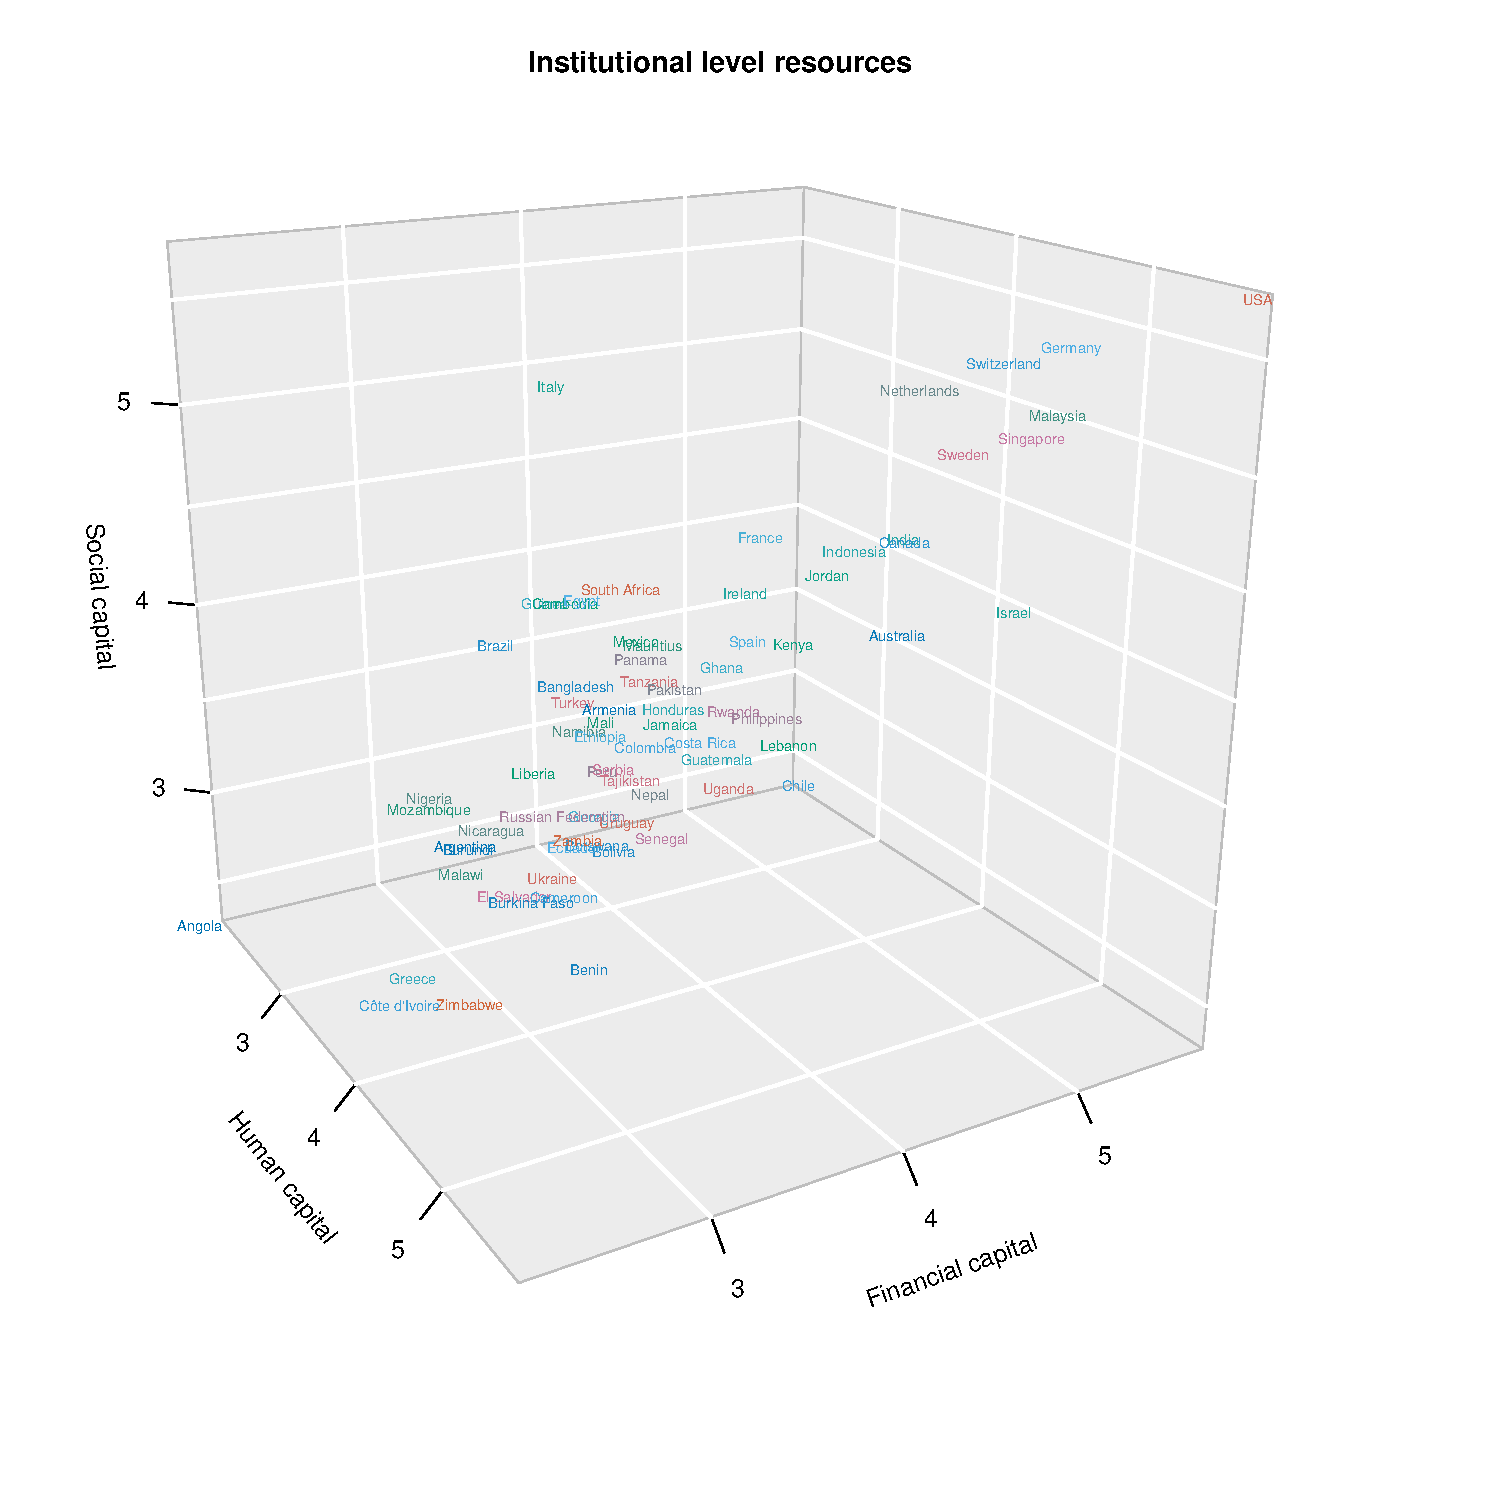
\includegraphics{Manuscript_files/figure-latex/unnamed-chunk-5-1} \caption{ }\label{fig:unnamed-chunk-5-1}
\end{figure}
\begin{figure}[!H]
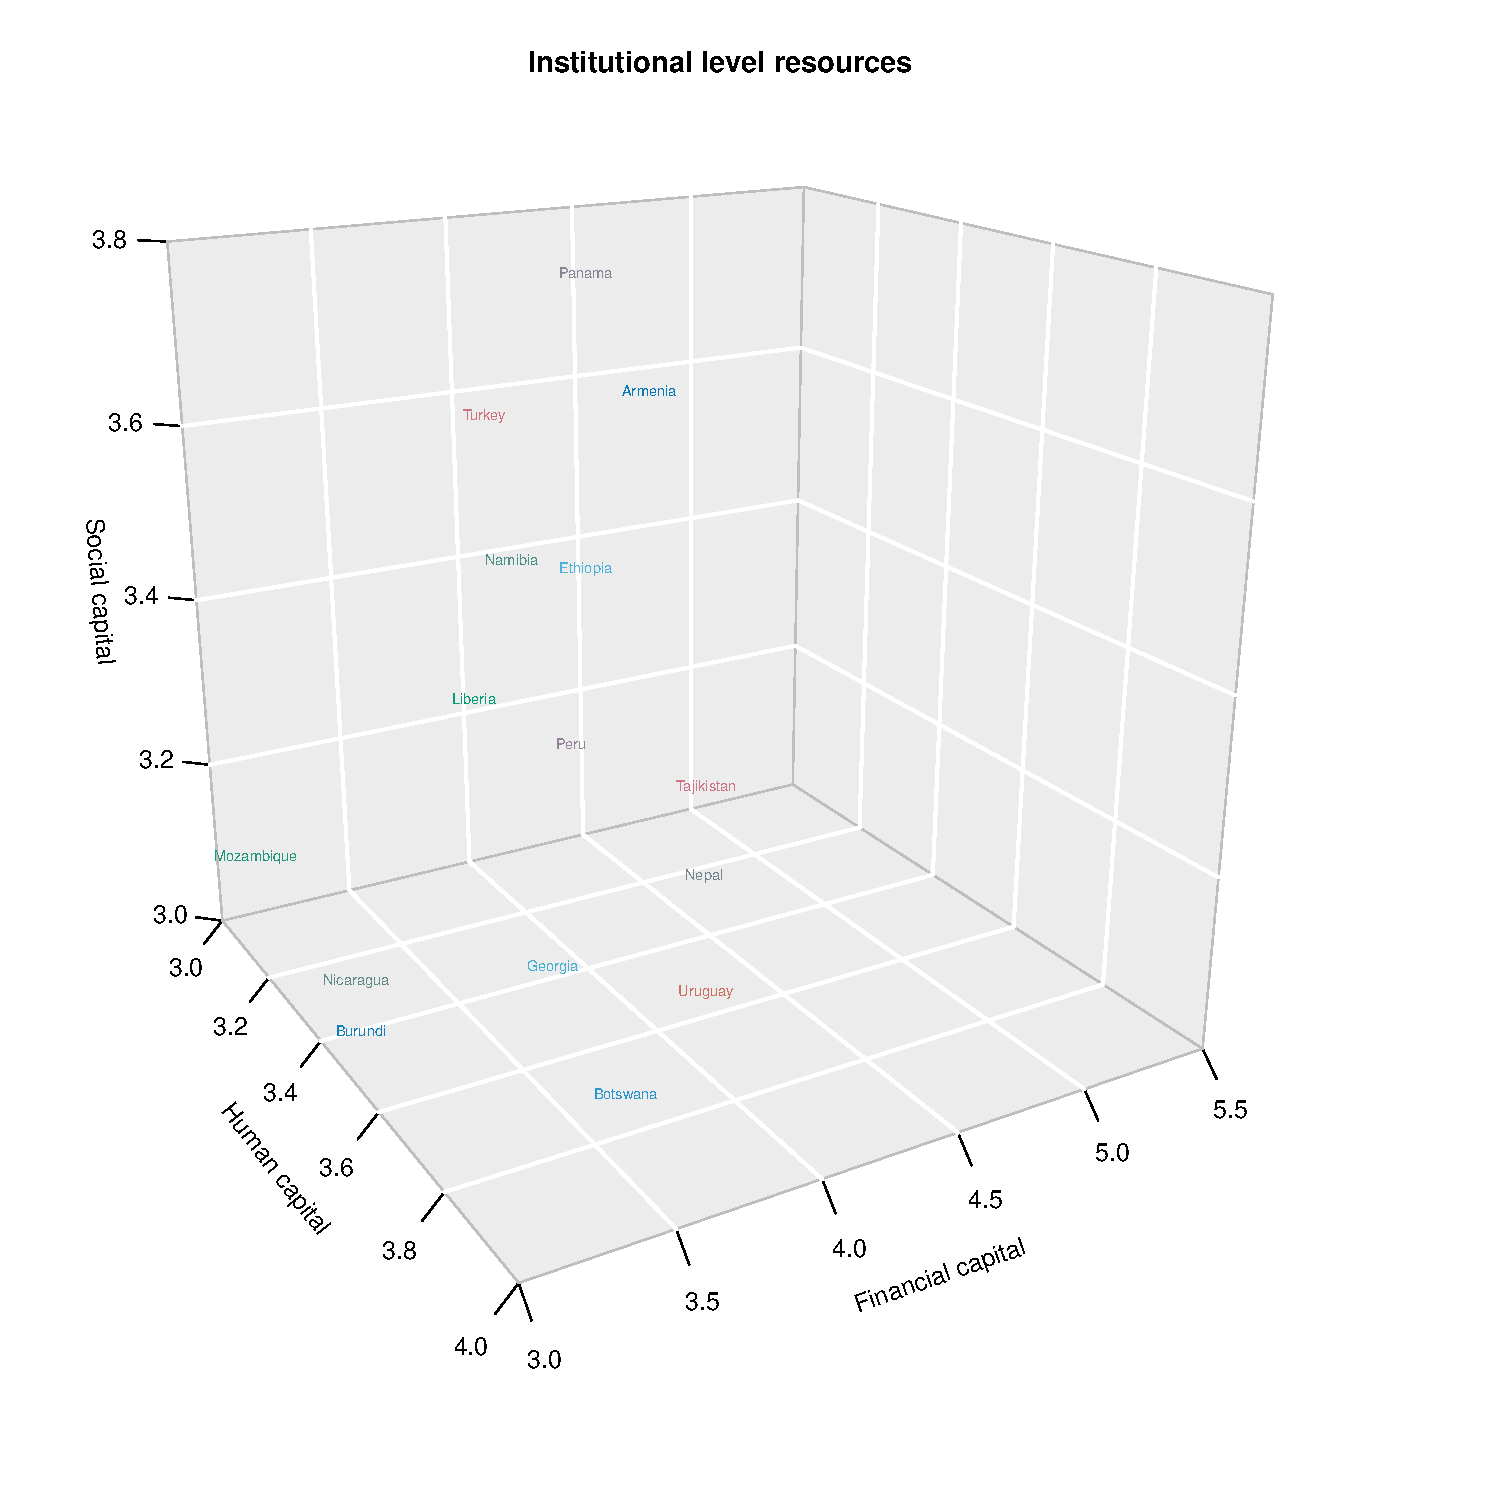
\includegraphics{Manuscript_files/figure-latex/unnamed-chunk-5-2} \caption{ }\label{fig:unnamed-chunk-5-2}
\end{figure}

\begin{figure}[!H]
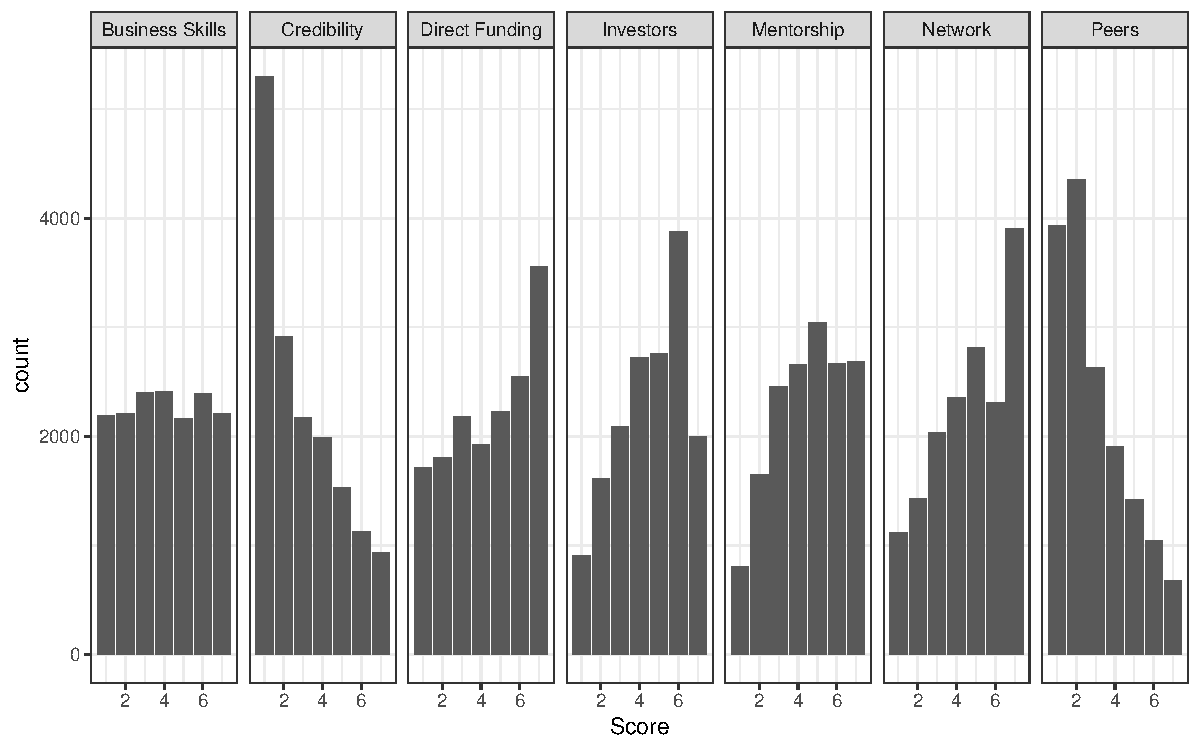
\includegraphics{Manuscript_files/figure-latex/unnamed-chunk-7-1} \caption{ }\label{fig:unnamed-chunk-7-1}
\end{figure}
\begin{figure}[!H]
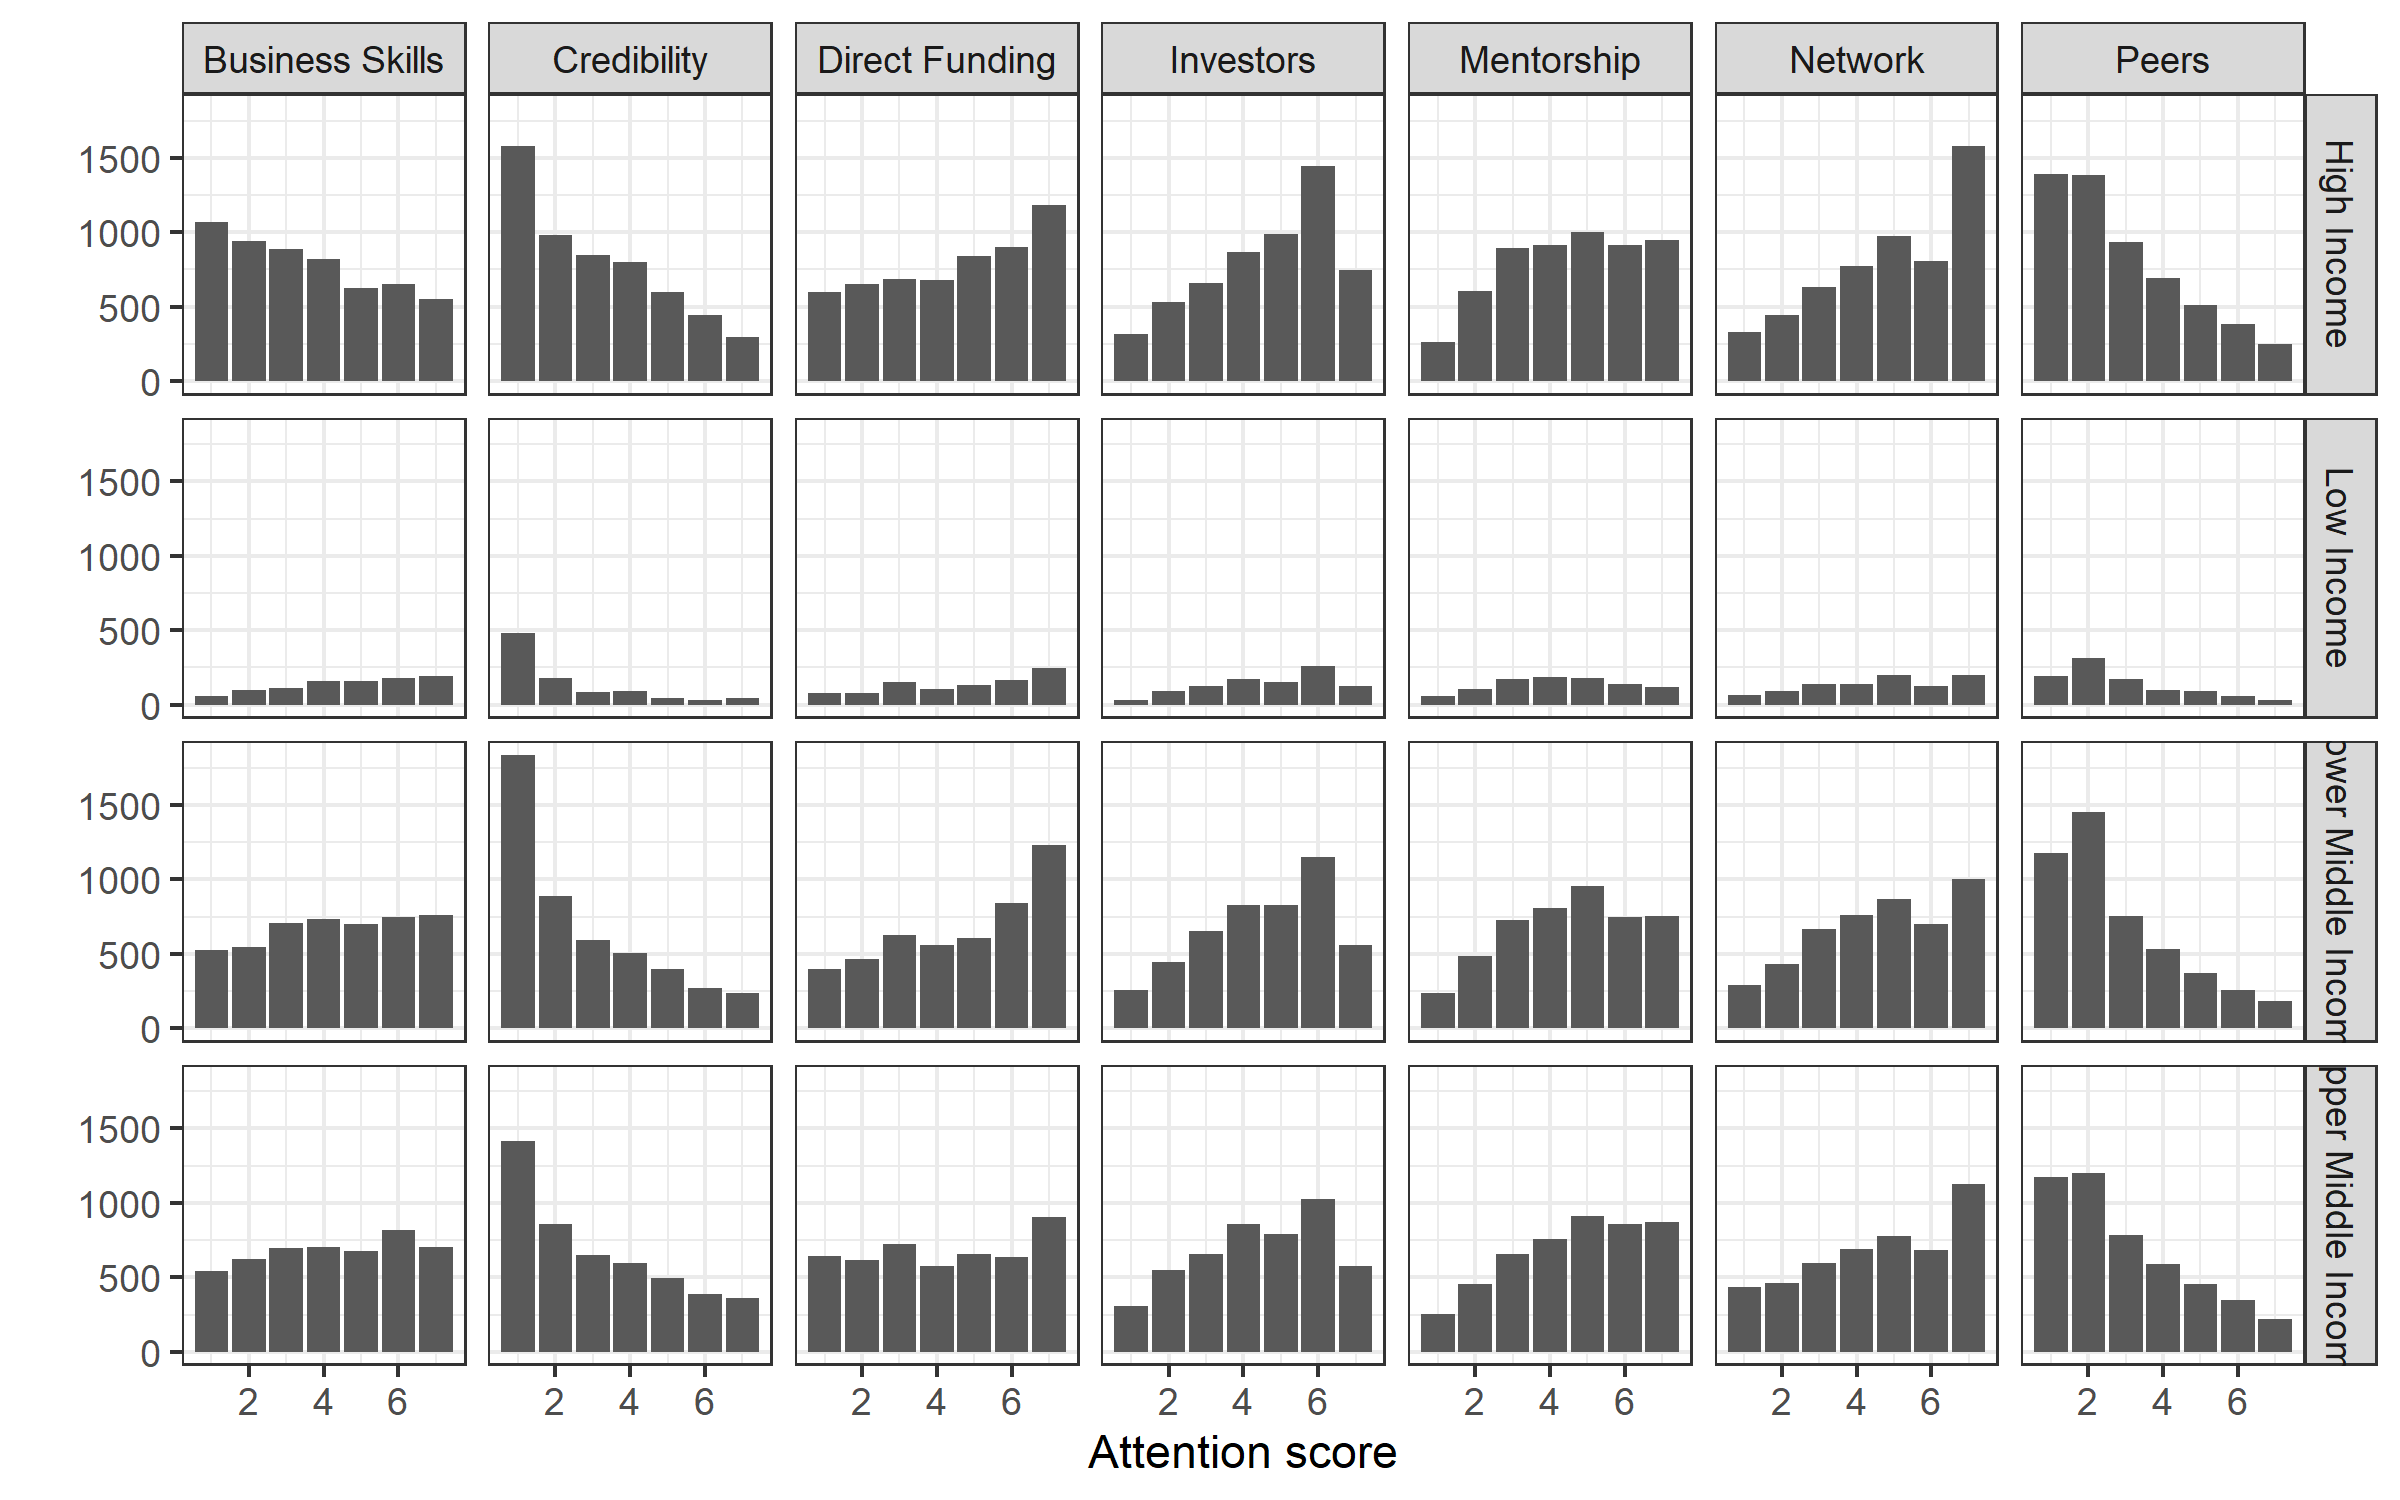
\includegraphics{Manuscript_files/figure-latex/unnamed-chunk-7-2} \caption{ }\label{fig:unnamed-chunk-7-2}
\end{figure}

\begin{figure}[!H]
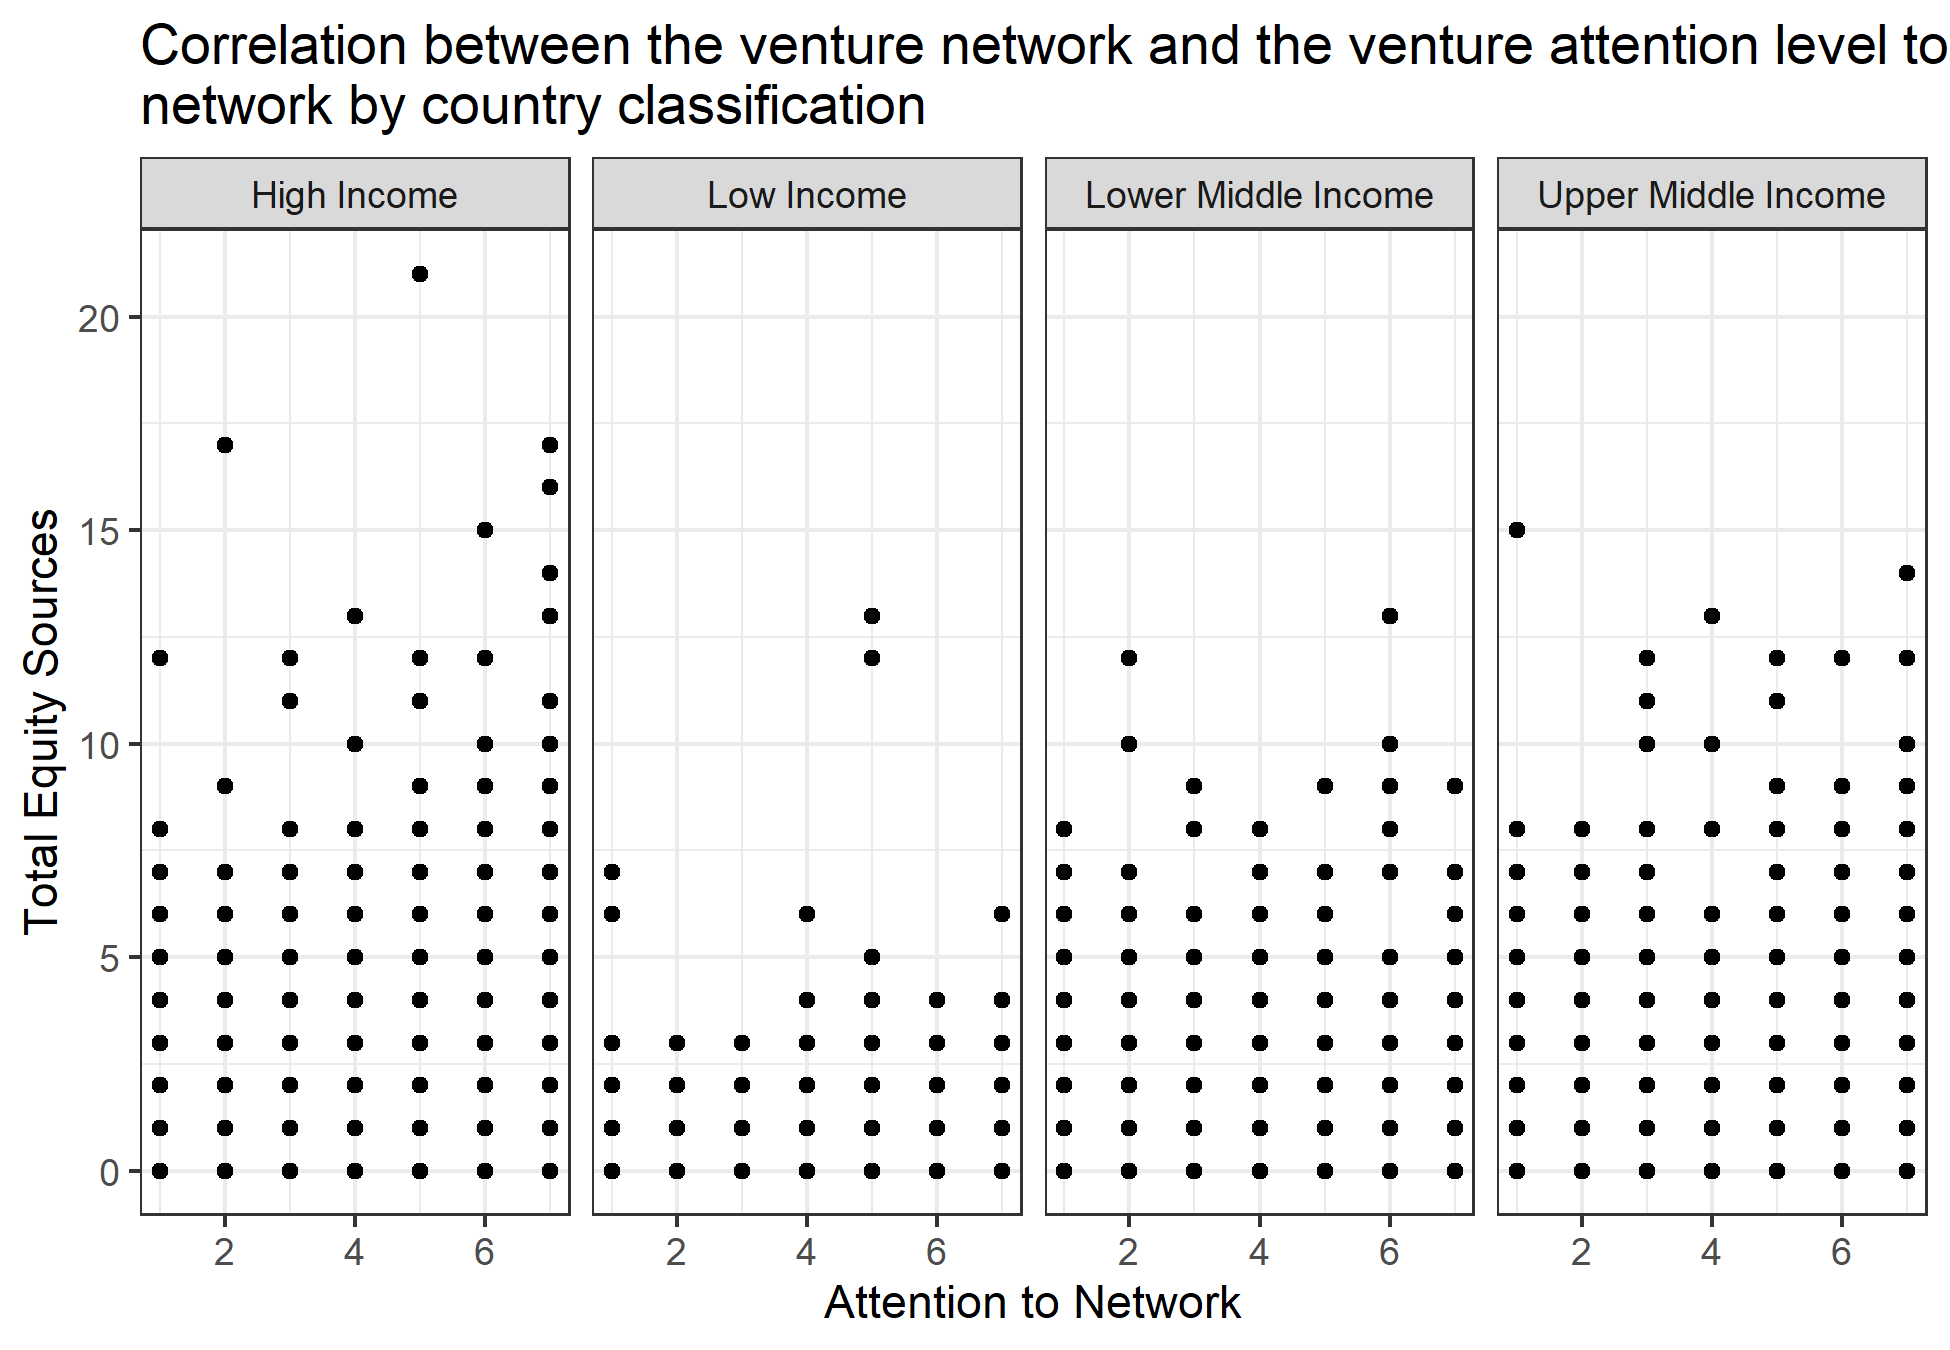
\includegraphics{Manuscript_files/figure-latex/unnamed-chunk-12-1} \caption{ }\label{fig:unnamed-chunk-12-1}
\end{figure}
\begin{figure}[!H]
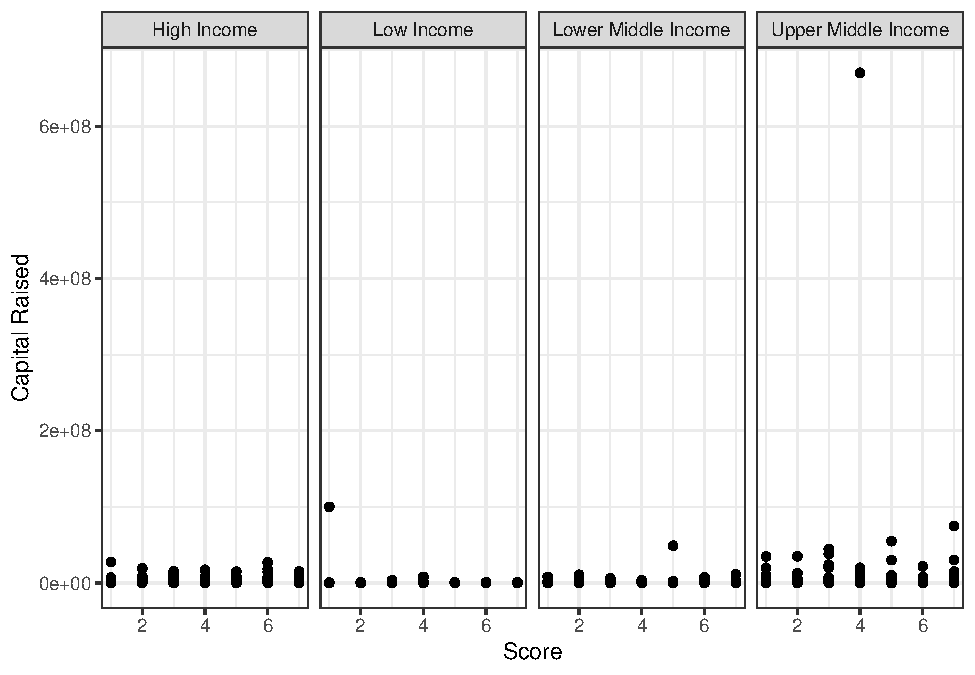
\includegraphics{Manuscript_files/figure-latex/unnamed-chunk-12-2} \caption{ }\label{fig:unnamed-chunk-12-2}
\end{figure}

\begin{table}

\caption{\label{tab:unnamed-chunk-18}Effect of attention to human capital on likelihood of participation}
\centering
\begin{tabular}[t]{l|l|l|l|l|l|l|l|l}
\hline
\multicolumn{1}{c|}{\em{ }} & \multicolumn{4}{c|}{\em{Model w/ controls}} & \multicolumn{4}{c}{\em{Model w/o controls}} \\
\cline{2-5} \cline{6-9}
  & $b$ & SE & $z$ & $p$ & $b$ & SE & $z$ & $p$\\
\hline
Intercept & -1.54 & 0.08 & -19.82 & 0.000 & -1.46 & 0.08 & -19.18 & 0.000\\
\hline
Attention to Human capital(AHC) & 0.09 & 0.07 & 1.24 & 0.215 & 0.11 & 0.07 & 1.54 & 0.123\\
\hline
\multicolumn{9}{l}{\textbf{Control variables}}\\
\hline
\hspace{1em}HCI & 0.01 & 0.01 & 1.46 & 0.144 & NA & NA & NA & NA\\
\hline
\hspace{1em}GC & 0.24 & 0.06 & 4.17 & 0.000 & NA & NA & NA & NA\\
\hline
\end{tabular}
\end{table}

\begin{table}

\caption{\label{tab:unnamed-chunk-18}Effect of congruency of venture attention and institutional level of human capital on likelihood of participation}
\centering
\begin{tabular}[t]{l|l|l|l|l|l|l|l|l}
\hline
\multicolumn{1}{c|}{\em{ }} & \multicolumn{4}{c|}{\em{Model w/ controls}} & \multicolumn{4}{c}{\em{Model w/o controls}} \\
\cline{2-5} \cline{6-9}
  & $b$ & SE & $z$ & $p$ & $b$ & SE & $z$ & $p$\\
\hline
Intercept & -0.94 & 0.53 & -1.80 & 0.073 & -0.85 & 0.53 & -1.61 & 0.108\\
\hline
AHC & 0.90 & 0.45 & 2.01 & 0.044 & 0.92 & 0.45 & 2.05 & 0.040\\
\hline
Ease of finding skilled employees & -0.13 & 0.12 & -1.11 & 0.269 & -0.14 & 0.12 & -1.14 & 0.253\\
\hline
AHCxEase of finding skilled employees & 0.01 & 0.01 & 1.37 & 0.171 & -0.17 & 0.10 & -1.79 & 0.074\\
\hline
\multicolumn{9}{l}{\textbf{Control variables}}\\
\hline
\hspace{1em}HCI & 0.24 & 0.06 & 4.06 & 0.000 & NA & NA & NA & NA\\
\hline
\hspace{1em}GC & -0.17 & 0.10 & -1.80 & 0.073 & NA & NA & NA & NA\\
\hline
\end{tabular}
\end{table}

\begin{table}

\caption{\label{tab:unnamed-chunk-18}Effect of attention to financial capital on likelihood of participation}
\centering
\begin{tabular}[t]{l|l|l|l|l|l|l|l|l}
\hline
\multicolumn{1}{c|}{\em{ }} & \multicolumn{4}{c|}{\em{Model w/ controls}} & \multicolumn{4}{c}{\em{Model w/o controls}} \\
\cline{2-5} \cline{6-9}
  & $b$ & SE & $z$ & $p$ & $b$ & SE & $z$ & $p$\\
\hline
Intercept & -1.53 & 0.08 & -19.55 & 0.000 & -1.45 & 0.08 & -18.82 & 0.000\\
\hline
Attention to Financial capital & -0.19 & 0.06 & -3.02 & 0.003 & -0.19 & 0.06 & -3.06 & 0.002\\
\hline
\multicolumn{9}{l}{\textbf{Control variables}}\\
\hline
\hspace{1em}HCI & 0.01 & 0.01 & 1.39 & 0.165 & NA & NA & NA & NA\\
\hline
\hspace{1em}GC & 0.25 & 0.06 & 4.34 & 0.000 & NA & NA & NA & NA\\
\hline
\end{tabular}
\end{table}

\begin{table}

\caption{\label{tab:unnamed-chunk-18}Effect of congruency of venture attention and institutional level (SME financing) of financial capital on likelihood of participation}
\centering
\begin{tabular}[t]{l|l|l|l|l|l|l|l|l}
\hline
\multicolumn{1}{c|}{\em{ }} & \multicolumn{4}{c|}{\em{Model w/ controls}} & \multicolumn{4}{c}{\em{Model w/o controls}} \\
\cline{2-5} \cline{6-9}
  & $b$ & SE & $z$ & $p$ & $b$ & SE & $z$ & $p$\\
\hline
Intercept & -1.43 & 0.43 & -3.35 & 0.001 & -1.35 & 0.43 & -3.11 & 0.002\\
\hline
AFC & -0.19 & 0.29 & -0.66 & 0.509 & -0.21 & 0.29 & -0.74 & 0.460\\
\hline
Financing of SMEs & -0.02 & 0.11 & -0.20 & 0.845 & -0.02 & 0.11 & -0.19 & 0.847\\
\hline
AFCxFinancing of SMEs & 0.01 & 0.01 & 1.30 & 0.193 & 0.00 & 0.07 & 0.05 & 0.959\\
\hline
\multicolumn{9}{l}{\textbf{Control variables}}\\
\hline
\hspace{1em}HCI & 0.25 & 0.06 & 4.25 & 0.000 & NA & NA & NA & NA\\
\hline
\hspace{1em}GC & 0.00 & 0.07 & -0.02 & 0.988 & NA & NA & NA & NA\\
\hline
\end{tabular}
\end{table}

\begin{table}

\caption{\label{tab:unnamed-chunk-18}Effect of congruency of venture attention and institutional level (VC) of financial capital on likelihood of participation}
\centering
\begin{tabular}[t]{l|l|l|l|l|l|l|l|l}
\hline
\multicolumn{1}{c|}{\em{ }} & \multicolumn{4}{c|}{\em{Model w/ controls}} & \multicolumn{4}{c}{\em{Model w/o controls}} \\
\cline{2-5} \cline{6-9}
  & $b$ & SE & $z$ & $p$ & $b$ & SE & $z$ & $p$\\
\hline
Intercept & -1.31 & 0.28 & -4.74 & 0.000 & -1.22 & 0.28 & -4.35 & 0.000\\
\hline
AFC & -0.23 & 0.20 & -1.17 & 0.244 & -0.24 & 0.20 & -1.24 & 0.217\\
\hline
VC Availability & -0.07 & 0.09 & -0.75 & 0.454 & -0.07 & 0.09 & -0.79 & 0.432\\
\hline
AFCxVC Availability & 0.01 & 0.01 & 1.31 & 0.190 & 0.01 & 0.05 & 0.28 & 0.778\\
\hline
\multicolumn{9}{l}{\textbf{Control variables}}\\
\hline
\hspace{1em}HCI & 0.24 & 0.06 & 4.23 & 0.000 & NA & NA & NA & NA\\
\hline
\hspace{1em}GC & 0.01 & 0.05 & 0.22 & 0.824 & NA & NA & NA & NA\\
\hline
\end{tabular}
\end{table}

\begin{table}

\caption{\label{tab:unnamed-chunk-18}Effect of congruency of venture attention and institutional level (Credit gaps) of financial capital on likelihood of participation}
\centering
\begin{tabular}[t]{l|l|l|l|l|l|l|l|l}
\hline
\multicolumn{1}{c|}{\em{ }} & \multicolumn{4}{c|}{\em{Model w/ controls}} & \multicolumn{4}{c}{\em{Model w/o controls}} \\
\cline{2-5} \cline{6-9}
  & $b$ & SE & $z$ & $p$ & $b$ & SE & $z$ & $p$\\
\hline
Intercept & -1.46 & 0.13 & -11.62 & 0.000 & -1.37 & 0.13 & -10.93 & 0.000\\
\hline
AFC & -0.20 & 0.10 & -1.91 & 0.056 & -0.21 & 0.10 & -1.99 & 0.047\\
\hline
Domestic Credit Gaps & 0.00 & 0.00 & -0.57 & 0.572 & 0.00 & 0.00 & -0.60 & 0.550\\
\hline
AFCxDomestic Credit Gaps & 0.01 & 0.01 & 1.30 & 0.192 & 0.00 & 0.00 & 0.15 & 0.882\\
\hline
\multicolumn{9}{l}{\textbf{Control variables}}\\
\hline
\hspace{1em}HCI & 0.25 & 0.06 & 4.24 & 0.000 & NA & NA & NA & NA\\
\hline
\hspace{1em}GC & 0.00 & 0.00 & 0.08 & 0.938 & NA & NA & NA & NA\\
\hline
\end{tabular}
\end{table}

\begin{table}

\caption{\label{tab:unnamed-chunk-18}Effect of attention to social capital on likelihood of participation}
\centering
\begin{tabular}[t]{l|l|l|l|l|l|l|l|l}
\hline
\multicolumn{1}{c|}{\em{ }} & \multicolumn{4}{c|}{\em{Model w/ controls}} & \multicolumn{4}{c}{\em{Model w/o controls}} \\
\cline{2-5} \cline{6-9}
  & $b$ & SE & $z$ & $p$ & $b$ & SE & $z$ & $p$\\
\hline
Intercept & -1.53 & 0.08 & -19.37 & 0.000 & -1.45 & 0.08 & -18.62 & 0.000\\
\hline
Attention to Social capital & 0.12 & 0.07 & 1.79 & 0.073 & 0.11 & 0.07 & 1.69 & 0.091\\
\hline
\multicolumn{9}{l}{\textbf{Control variables}}\\
\hline
\hspace{1em}HCI & 0.01 & 0.01 & 1.29 & 0.197 & NA & NA & NA & NA\\
\hline
\hspace{1em}GC & 0.25 & 0.06 & 4.42 & 0.000 & NA & NA & NA & NA\\
\hline
\end{tabular}
\end{table}

\begin{table}

\caption{\label{tab:unnamed-chunk-18}Effect of congruency of venture attention and institutional level of social capital on likelihood of participation}
\centering
\begin{tabular}[t]{l|l|l|l|l|l|l|l|l}
\hline
\multicolumn{1}{c|}{\em{ }} & \multicolumn{4}{c|}{\em{Model w/ controls}} & \multicolumn{4}{c}{\em{Model w/o controls}} \\
\cline{2-5} \cline{6-9}
  & $b$ & SE & $z$ & $p$ & $b$ & SE & $z$ & $p$\\
\hline
Intercept & -0.89 & 0.41 & -2.16 & 0.031 & -0.78 & 0.42 & -1.87 & 0.061\\
\hline
ASC & 0.06 & 0.35 & 0.19 & 0.852 & 0.06 & 0.35 & 0.18 & 0.860\\
\hline
State of cluster development & -0.16 & 0.10 & -1.52 & 0.128 & -0.17 & 0.11 & -1.56 & 0.119\\
\hline
ASCxState of cluster development & 0.01 & 0.01 & 1.22 & 0.223 & 0.01 & 0.08 & 0.15 & 0.883\\
\hline
\multicolumn{9}{l}{\textbf{Control variables}}\\
\hline
\hspace{1em}HCI & 0.25 & 0.06 & 4.30 & 0.000 & NA & NA & NA & NA\\
\hline
\hspace{1em}GC & 0.01 & 0.08 & 0.16 & 0.876 & NA & NA & NA & NA\\
\hline
\end{tabular}
\end{table}

\begin{table}

\caption{\label{tab:unnamed-chunk-21}Effect on total employees}
\centering
\begin{tabular}[t]{l|l|l|l|l|l|l}
\hline
\multicolumn{1}{c|}{\em{ }} & \multicolumn{3}{c|}{\em{Congruence}} & \multicolumn{3}{c}{\em{AHC only}} \\
\cline{2-4} \cline{5-7}
  & $b$ & SE & $t$ & $b$ & SE & $t$\\
\hline
Intercept & -1,955.91 & 3,599.05 & -0.54 & 762.25 & 502.25 & 1.52\\
\hline
AHC & -10,174.65 & 16,704.03 & -0.61 & 2,955.97 & 2,238.11 & 1.32\\
\hline
Ease of finding skilled employees & 641.03 & 813.08 & 0.79 & NA & NA & NA\\
\hline
AHCxEase of finding skilled employees & 3,118.93 & 3,842.90 & 0.81 & NA & NA & NA\\
\hline
\end{tabular}
\end{table}

\begin{table}

\caption{\label{tab:unnamed-chunk-21}Effect on capital raised}
\centering
\begin{tabular}[t]{l|l|l|l|l|l|l}
\hline
\multicolumn{1}{c|}{\em{ }} & \multicolumn{3}{c|}{\em{Congruence}} & \multicolumn{3}{c}{\em{AFC only}} \\
\cline{2-4} \cline{5-7}
  & $b$ & SE & $t$ & $b$ & SE & $t$\\
\hline
Intercept & -4,884.58 & 444,377.03 & -0.01 & 223,507.35 & 80,002.22 & 2.79\\
\hline
AFC & -191,023.97 & 590,674.78 & -0.32 & -62,834.51 & 130,477.16 & -0.48\\
\hline
Financing of SMEs & 59,478.10 & 112,868.11 & 0.53 & NA & NA & NA\\
\hline
AFCxFinancing of SMEs & 31,388.20 & 134,941.74 & 0.23 & NA & NA & NA\\
\hline
\end{tabular}
\end{table}

\begin{table}

\caption{\label{tab:unnamed-chunk-21}Effect on capital raised}
\centering
\begin{tabular}[t]{l|l|l|l}
\hline
  & $b$ & SE & $t$\\
\hline
Intercept & 66,014.34 & 285,161.56 & 0.23\\
\hline
AFC & -205,432.60 & 401,457.67 & -0.51\\
\hline
VC Availability & 51,857.72 & 88,842.97 & 0.58\\
\hline
AFCxVC Availability & 41,162.01 & 104,375.22 & 0.39\\
\hline
\end{tabular}
\end{table}

\begin{table}

\caption{\label{tab:unnamed-chunk-21}Effect on capital raised}
\centering
\begin{tabular}[t]{l|l|l|l}
\hline
  & $b$ & SE & $t$\\
\hline
Intercept & 190,992.97 & 128,015.34 & 1.49\\
\hline
AFC & -121,351.86 & 210,077.95 & -0.58\\
\hline
Domestic Credit Gaps & 572.94 & 1,620.34 & 0.35\\
\hline
AFCxDomestic Credit Gaps & 768.35 & 1,952.74 & 0.39\\
\hline
\end{tabular}
\end{table}

\begin{table}

\caption{\label{tab:unnamed-chunk-21}Effect on sources of capital}
\centering
\begin{tabular}[t]{l|l|l|l|l|l|l}
\hline
\multicolumn{1}{c|}{\em{ }} & \multicolumn{3}{c|}{\em{Congruence}} & \multicolumn{3}{c}{\em{ASC only}} \\
\cline{2-4} \cline{5-7}
  & $b$ & SE & $t$ & $b$ & SE & $t$\\
\hline
Intercept & -0.28 & 0.21 & -1.30 & 0.58 & 0.04 & 13.35\\
\hline
ASC & -0.60 & 0.25 & -2.45 & 0.06 & 0.05 & 1.35\\
\hline
State of cluster development & 0.22 & 0.05 & 4.09 & NA & NA & NA\\
\hline
ASCxState of cluster development & 0.17 & 0.06 & 2.94 & NA & NA & NA\\
\hline
\end{tabular}
\end{table}

\begin{table}

\caption{\label{tab:unnamed-chunk-24}Effect on revenues}
\centering
\fontsize{8}{10}\selectfont
\begin{tabular}[t]{l|l|l|l|l|l|l}
\hline
\multicolumn{1}{c|}{\em{ }} & \multicolumn{3}{c|}{\em{Congruence}} & \multicolumn{3}{c}{\em{AHC only}} \\
\cline{2-4} \cline{5-7}
  & $b$ & SE & $t$ & $b$ & SE & $t$\\
\hline
Intercept & 5,033,422.50 & 8,779,342.42 & 0.57 & 2,061,441.83 & 1,172,119.94 & 1.76\\
\hline
AHC & 12,174,047.87 & 13,178,734.99 & 0.92 & 1,309,266.88 & 2,015,947.62 & 0.65\\
\hline
Ease of finding skilled employees & -677,452.53 & 1,991,735.94 & -0.34 & NA & NA & NA\\
\hline
AHCxEase of finding skilled employees & -2,337,599.95 & 2,803,682.74 & -0.83 & NA & NA & NA\\
\hline
\end{tabular}
\end{table}

\begin{table}

\caption{\label{tab:unnamed-chunk-24}Effect on revenues}
\centering
\fontsize{8}{10}\selectfont
\begin{tabular}[t]{l|l|l|l|l|l|l}
\hline
\multicolumn{1}{c|}{\em{ }} & \multicolumn{3}{c|}{\em{Congruence}} & \multicolumn{3}{c}{\em{AFC only}} \\
\cline{2-4} \cline{5-7}
  & $b$ & SE & $t$ & $b$ & SE & $t$\\
\hline
Intercept & 1,091,420.63 & 7,860,432.48 & 0.14 & 1,812,535.35 & 1,024,606.34 & 1.77\\
\hline
AFC & -3,691,743.30 & 26,035,557.36 & -0.14 & -5,533,248.45 & 3,452,852.29 & -1.60\\
\hline
Financing of SMEs & 220,995.73 & 4,112,461.43 & 0.05 & NA & NA & NA\\
\hline
VC Availability & -20,625.49 & 3,293,858.39 & -0.01 & NA & NA & NA\\
\hline
Domestic Credit Gaps & 112.62 & 29,302.15 & 0.00 & NA & NA & NA\\
\hline
AFCxFinancing of SMEs & -450,299.34 & 13,580,706.25 & -0.03 & NA & NA & NA\\
\hline
AFCxVC Availability & -265,392.62 & 10,933,461.08 & -0.02 & NA & NA & NA\\
\hline
AFCxDomestic Credit Gaps & 5,897.33 & 98,489.71 & 0.06 & NA & NA & NA\\
\hline
\end{tabular}
\end{table}

\begin{table}

\caption{\label{tab:unnamed-chunk-24}Effect on revenues}
\centering
\fontsize{8}{10}\selectfont
\begin{tabular}[t]{l|l|l|l|l|l|l}
\hline
\multicolumn{1}{c|}{\em{ }} & \multicolumn{3}{c|}{\em{Congruence}} & \multicolumn{3}{c}{\em{ASC only}} \\
\cline{2-4} \cline{5-7}
  & $b$ & SE & $t$ & $b$ & SE & $t$\\
\hline
Intercept & 3,743,005.06 & 6,777,362.02 & 0.55 & 2,072,186.10 & 1,151,987.55 & 1.80\\
\hline
ASC & -5,807,873.96 & 17,276,071.97 & -0.34 & -2,440,778.66 & 2,993,083.09 & -0.82\\
\hline
State of cluster development & -401,960.58 & 1,679,258.60 & -0.24 & NA & NA & NA\\
\hline
ASCxState of cluster development & 825,623.52 & 4,199,015.96 & 0.20 & NA & NA & NA\\
\hline
\end{tabular}
\end{table}

\hypertarget{results-and-discussion}{%
\section{Results and Discussion}\label{results-and-discussion}}

\textbf{Resource mobilization}

I find no support for hypothesis 1, with exception for certain resources. Specifically, Table 1 shows that an increase in venture attention to human capital causes an increase in the venture's likelihood to participate to the acceleration program and mobilize resources. However, this effect is not statistically significant. The model is robust to the addition of control variables. Similarly, table 7 show that an increase in venture to attention social capital causes an increase in the venture's likelihood to mobilize resources within the acceleration program. These effects are not statistically signification. Table 3 on the other hand, show that an increase in venture attention to social capital results in a significant decrease in the venture's likelihood to mobilize resources. This shows that early stage ventures applying to accelerator programs benefit the most if they first focus on mobilizing human and social capital resources before turning attention to financial capital. To examine our hypotheses exploring these same relationships within the institutional context of the venture, we turn to tables 2, 4, 5, 6, and 8. When I interact the venture level attention to human capital with the institutional level human capital (Table 2), I find that attention to this resource results in a significant increase in the likelihood to mobilize resources within the accelerator program (\(b = 0.9\)), and the model is robust to control variables. In contrast, tables 3 to 5 show that attention to financial capital has a non-significant effect on the venture's likelihood to mobilize resources regardless of the institutional context. We find the same results whether we consider institutional level capital for SMEs, VC oriented ventures, or ventures seeking loans and other forms of financing from financial establishments. This is in line with our initial finding that human and social capital should garner the attention of ventures seeking resources in their early stage from incubators and accelerators. Finally, table 8 shows us that the congruency of venture attention and the institutional level of social capital does not have any significant effect on the venture's likelihood to mobilize resources.

This first part of the analysis focuses on resource mobilization within accelerator programs and explores the relationship between venture attention to a certain type of resources and its influence on the venture's likelihood to participate to the program. I find that social and human capital are the key resources that should be on the venture's radar in their early stage of strategy formation. I then investigate the impact of the congruency between the venture attention and the institutional level capital to better understand these relationships within their institutional context. I find that human capital is not only one of the key resources to focus on but it becomes even more important if it aligns with the venture's country to provide skillful human resources.

\textbf{Resource acquisition}

Similar to hypothesis 1, I find no support for the second hypothesis. Table 9 shows the impact of venture attention to human capital and its congruency level with the institutional capital on the acquisition of human capital (total number of employees) post-acceleration program. I find no significant effect in the two models. Tables 10 to 12 show the impact of venture attention to financial capital and its congruency level with the institutional capital on the acquisition of financial capital (capital raised in USD) post-acceleration program. I find no significant effect in the two models. Finally, table 13 shows the the impact of venture attention to social capital and its congruency level with the institutional capital on the acquisition of social capital (sources of capital) post-acceleration program. I find no significant effect in the two models.

It is important to highlight here, that not only I find no significant effect but also all the coefficients are negative. This negative effect on resource acquisition post-acceleration program can be interpreted economically, as an opportunity cost. Ventures that succeed in mobilizing resources put their time and efforts into acquiring business skills, developing their network, and seeking funding resources. While these efforts might result in resource acquisition, over the long-term, we would not be able to observe this within a year or two post resource mobilization. This is a key limitation of our data and analysis.

\textbf{Performance}

Based on the results of resource acquisition we would expect similar results for venture performance (hypothesis 3) since revenues are often accumulated post resource acquisition. We can consider this part of the analysis as a robustness check for the previous analysis on resource acquisition. Tables 14 to 16 confirm these expectations. I find only null effects of the impact of venture attention to a resource and its congruency level with the institutional level of the resource on performance (measured based on firm revenues) post acceleration program.

There are several channels to interpret the results of all three outcomes. The most plausible explanation is that at their early stages of venturing, entrepreneurs do not have to align their attention to resources with the availability of resources in their institutional environment. However, their attention to internal human capital (i.e.~building their own business skills) becomes important if we consider the outcome as being selection to an incubation program instead to mobilize resources and prepare for long-term resource acquisition. Resource acquisition is a long-term goal and that is why I do not see any effects in the short term (2 years post acceleration). In contrast, selection to an incubation program is a short-term goal that opens the door for the long-term effects and that is how ventures in our sample should approach their resource base strategy (i.e.~mobilization first and acquisition would follow).

\newpage

\hypertarget{references}{%
\section{References}\label{references}}

\begingroup
\setlength{\parindent}{-0.5in}
\setlength{\leftskip}{0.5in}

\hypertarget{refs}{}
\leavevmode\hypertarget{ref-R-papaja}{}%
Aust, F., \& Barth, M. (2020). \emph{papaja: Create APA manuscripts with R Markdown}. Retrieved from \url{https://github.com/crsh/papaja}

\leavevmode\hypertarget{ref-R-Matrix}{}%
Bates, D., \& Maechler, M. (2019). \emph{Matrix: Sparse and dense matrix classes and methods}. Retrieved from \url{https://CRAN.R-project.org/package=Matrix}

\leavevmode\hypertarget{ref-R-lme4}{}%
Bates, D., Mächler, M., Bolker, B., \& Walker, S. (2015). Fitting linear mixed-effects models using lme4. \emph{Journal of Statistical Software}, \emph{67}(1), 1--48. \url{https://doi.org/10.18637/jss.v067.i01}

\leavevmode\hypertarget{ref-R-preprocessCore}{}%
Bolstad, B. (2020). \emph{PreprocessCore: A collection of pre-processing functions}. Retrieved from \url{https://github.com/bmbolstad/preprocessCore}

\leavevmode\hypertarget{ref-R-rio}{}%
Chan, C.-h., Chan, G. C., Leeper, T. J., \& Becker, J. (2018). \emph{Rio: A swiss-army knife for data file i/o}.

\leavevmode\hypertarget{ref-colombo2005founders}{}%
Colombo, M. G., \& Grilli, L. (2005). Founders' human capital and the growth of new technology-based firms: A competence-based view. \emph{Research Policy}, \emph{34}(6), 795--816.

\leavevmode\hypertarget{ref-R-plm_a}{}%
Croissant, Y., \& Millo, G. (2008). Panel data econometrics in R: The plm package. \emph{Journal of Statistical Software}, \emph{27}(2), 1--43. \url{https://doi.org/10.18637/jss.v027.i02}

\leavevmode\hypertarget{ref-dimov2005human}{}%
Dimov, D. P., \& Shepherd, D. A. (2005). Human capital theory and venture capital firms: Exploring ``home runs'' and ``strike outs''. \emph{Journal of Business Venturing}, \emph{20}(1), 1--21.

\leavevmode\hypertarget{ref-estrin2016human}{}%
Estrin, S., Mickiewicz, T., \& Stephan, U. (2016). Human capital in social and commercial entrepreneurship. \emph{Journal of Business Venturing}, \emph{31}(4), 449--467.

\leavevmode\hypertarget{ref-R-janitor}{}%
Firke, S. (2020). \emph{Janitor: Simple tools for examining and cleaning dirty data}. Retrieved from \url{https://CRAN.R-project.org/package=janitor}

\leavevmode\hypertarget{ref-gebauer2009attention}{}%
Gebauer, H. (2009). An attention-based view on service orientation in the business strategy of manufacturing companies. \emph{Journal of Managerial Psychology}.

\leavevmode\hypertarget{ref-R-lubridate}{}%
Grolemund, G., \& Wickham, H. (2011). Dates and times made easy with lubridate. \emph{Journal of Statistical Software}, \emph{40}(3), 1--25. Retrieved from \url{http://www.jstatsoft.org/v40/i03/}

\leavevmode\hypertarget{ref-hansen2012removing}{}%
Hansen, K. D., Irizarry, R. A., \& Wu, Z. (2012). Removing technical variability in rna-seq data using conditional quantile normalization. \emph{Biostatistics}, \emph{13}(2), 204--216.

\leavevmode\hypertarget{ref-R-purrr}{}%
Henry, L., \& Wickham, H. (2020). \emph{Purrr: Functional programming tools}. Retrieved from \url{https://CRAN.R-project.org/package=purrr}

\leavevmode\hypertarget{ref-hochberg2007whom}{}%
Hochberg, Y. V., Ljungqvist, A., \& Lu, Y. (2007). Whom you know matters: Venture capital networks and investment performance. \emph{The Journal of Finance}, \emph{62}(1), 251--301.

\leavevmode\hypertarget{ref-holburn2010political}{}%
Holburn, G. L., \& Zelner, B. A. (2010). Political capabilities, policy risk, and international investment strategy: Evidence from the global electric power generation industry. \emph{Strategic Management Journal}, \emph{31}(12), 1290--1315.

\leavevmode\hypertarget{ref-khanna1997focused}{}%
Khanna, T., \& Palepu, K. (1997). Why focused strategies may be wrong for emerging markets. \emph{Harvard Business Review}, \emph{75}, 41--54.

\leavevmode\hypertarget{ref-khanna2001estimating}{}%
Khanna, T., \& Rivkin, J. W. (2001). Estimating the performance effects of business groups in emerging markets. \emph{Strategic Management Journal}, \emph{22}(1), 45--74.

\leavevmode\hypertarget{ref-kock2001strategy}{}%
Kock, C. J., \& Guillén, M. F. (2001). Strategy and structure in developing countries: Business groups as an evolutionary response to opportunities for unrelated diversification. \emph{Industrial and Corporate Change}, \emph{10}(1), 77--113.

\leavevmode\hypertarget{ref-R-caret}{}%
Kuhn, M. (2020). \emph{Caret: Classification and regression training}. Retrieved from \url{https://CRAN.R-project.org/package=caret}

\leavevmode\hypertarget{ref-R-lmerTest}{}%
Kuznetsova, A., Brockhoff, P. B., \& Christensen, R. H. B. (2017). lmerTest package: Tests in linear mixed effects models. \emph{Journal of Statistical Software}, \emph{82}(13), 1--26. \url{https://doi.org/10.18637/jss.v082.i13}

\leavevmode\hypertarget{ref-R-sjPlot}{}%
Lüdecke, D. (2020). \emph{SjPlot: Data visualization for statistics in social science}. Retrieved from \url{https://CRAN.R-project.org/package=sjPlot}

\leavevmode\hypertarget{ref-R-plm_b}{}%
Millo, G. (2017). Robust standard error estimators for panel models: A unifying approach. \emph{Journal of Statistical Software}, \emph{82}(3), 1--27. \url{https://doi.org/10.18637/jss.v082.i03}

\leavevmode\hypertarget{ref-R-XLConnect}{}%
Mirai Solutions GmbH. (2020). \emph{XLConnect: Excel connector for r}. Retrieved from \url{https://CRAN.R-project.org/package=XLConnect}

\leavevmode\hypertarget{ref-R-tibble}{}%
Müller, K., \& Wickham, H. (2020). \emph{Tibble: Simple data frames}. Retrieved from \url{https://CRAN.R-project.org/package=tibble}

\leavevmode\hypertarget{ref-north1990institutions}{}%
North, D. C., \& others. (1990). \emph{Institutions, institutional change and economic performance}. Cambridge university press.

\leavevmode\hypertarget{ref-R-foreign}{}%
R Core Team. (2020a). \emph{Foreign: Read data stored by 'minitab', 's', 'sas', 'spss', 'stata', 'systat', 'weka', 'dBase', ...} Retrieved from \url{https://CRAN.R-project.org/package=foreign}

\leavevmode\hypertarget{ref-R-base}{}%
R Core Team. (2020b). \emph{R: A language and environment for statistical computing}. Vienna, Austria: R Foundation for Statistical Computing. Retrieved from \url{https://www.R-project.org/}

\leavevmode\hypertarget{ref-R-psych}{}%
Revelle, W. (2019). \emph{Psych: Procedures for psychological, psychometric, and personality research}. Evanston, Illinois: Northwestern University. Retrieved from \url{https://CRAN.R-project.org/package=psych}

\leavevmode\hypertarget{ref-R-lattice}{}%
Sarkar, D. (2008). \emph{Lattice: Multivariate data visualization with r}. New York: Springer. Retrieved from \url{http://lmdvr.r-forge.r-project.org}

\leavevmode\hypertarget{ref-shane2002organizational}{}%
Shane, S., \& Stuart, T. (2002). Organizational endowments and the performance of university start-ups. \emph{Management Science}, \emph{48}(1), 154--170.

\leavevmode\hypertarget{ref-simon1947comment}{}%
Simon, H. A. (1947). A comment on" the science of public administration". \emph{Public Administration Review}, \emph{7}(3), 200--203.

\leavevmode\hypertarget{ref-R-plot3D}{}%
Soetaert, K. (2019). \emph{Plot3D: Plotting multi-dimensional data}. Retrieved from \url{https://CRAN.R-project.org/package=plot3D}

\leavevmode\hypertarget{ref-R-reshape2}{}%
Wickham, H. (2007). Reshaping data with the reshape package. \emph{Journal of Statistical Software}, \emph{21}(12), 1--20. Retrieved from \url{http://www.jstatsoft.org/v21/i12/}

\leavevmode\hypertarget{ref-R-ggplot2}{}%
Wickham, H. (2016). \emph{Ggplot2: Elegant graphics for data analysis}. Springer-Verlag New York. Retrieved from \url{https://ggplot2.tidyverse.org}

\leavevmode\hypertarget{ref-R-stringr}{}%
Wickham, H. (2019). \emph{Stringr: Simple, consistent wrappers for common string operations}. Retrieved from \url{https://CRAN.R-project.org/package=stringr}

\leavevmode\hypertarget{ref-R-forcats}{}%
Wickham, H. (2020). \emph{Forcats: Tools for working with categorical variables (factors)}. Retrieved from \url{https://CRAN.R-project.org/package=forcats}

\leavevmode\hypertarget{ref-R-tidyverse}{}%
Wickham, H., Averick, M., Bryan, J., Chang, W., McGowan, L. D., François, R., \ldots{} Yutani, H. (2019). Welcome to the tidyverse. \emph{Journal of Open Source Software}, \emph{4}(43), 1686. \url{https://doi.org/10.21105/joss.01686}

\leavevmode\hypertarget{ref-R-readxl}{}%
Wickham, H., \& Bryan, J. (2019). \emph{Readxl: Read excel files}. Retrieved from \url{https://CRAN.R-project.org/package=readxl}

\leavevmode\hypertarget{ref-R-dplyr}{}%
Wickham, H., François, R., Henry, L., \& Müller, K. (2020). \emph{Dplyr: A grammar of data manipulation}. Retrieved from \url{https://CRAN.R-project.org/package=dplyr}

\leavevmode\hypertarget{ref-R-tidyr}{}%
Wickham, H., \& Henry, L. (2020). \emph{Tidyr: Tidy messy data}. Retrieved from \url{https://CRAN.R-project.org/package=tidyr}

\leavevmode\hypertarget{ref-R-readr}{}%
Wickham, H., Hester, J., \& Francois, R. (2018). \emph{Readr: Read rectangular text data}. Retrieved from \url{https://CRAN.R-project.org/package=readr}

\leavevmode\hypertarget{ref-R-haven}{}%
Wickham, H., \& Miller, E. (2020). \emph{Haven: Import and export 'spss', 'stata' and 'sas' files}. Retrieved from \url{https://CRAN.R-project.org/package=haven}

\leavevmode\hypertarget{ref-R-knitr}{}%
Xie, Y. (2015). \emph{Dynamic documents with R and knitr} (2nd ed.). Boca Raton, Florida: Chapman; Hall/CRC. Retrieved from \url{https://yihui.org/knitr/}

\leavevmode\hypertarget{ref-R-EFAutilities}{}%
Zhang, G., Jiang, G., Hattori, M., \& Trichtinger, L. (2019). \emph{EFAutilities: Utility functions for exploratory factor analysis}. Retrieved from \url{https://CRAN.R-project.org/package=EFAutilities}

\endgroup


\end{document}
